\documentclass[a4paper]{article}
\usepackage[utf8x]{inputenc}
\usepackage[T1,T2A]{fontenc}
\usepackage[russian]{babel}
\usepackage{hyperref}
\usepackage{indentfirst}
\usepackage{listings}
\usepackage{color}
\usepackage{here}
\usepackage{array}
\usepackage{multirow}
\usepackage{graphicx}

\usepackage{caption}
\renewcommand{\lstlistingname}{Программа} % заголовок листингов кода

\usepackage{amssymb,amsfonts,amsmath} % Математика
\numberwithin{equation}{section} % Формула вида секция.номер

\usepackage{listings}
\lstset{ %
extendedchars=\true,
keepspaces=true,
language=C,						% choose the language of the code
basicstyle=\footnotesize,		% the size of the fonts that are used for the code
numbers=left,					% where to put the line-numbers
numberstyle=\footnotesize,		% the size of the fonts that are used for the line-numbers
stepnumber=1,					% the step between two line-numbers. If it is 1 each line will be numbered
numbersep=5pt,					% how far the line-numbers are from the code
backgroundcolor=\color{white},	% choose the background color. You must add \usepackage{color}
showspaces=false				% show spaces adding particular underscores
showstringspaces=false,			% underline spaces within strings
showtabs=false,					% show tabs within strings adding particular underscores
frame=single,           		% adds a frame around the code
tabsize=2,						% sets default tabsize to 2 spaces
captionpos=b,					% sets the caption-position to bottom
breaklines=true,				% sets automatic line breaking
breakatwhitespace=false,		% sets if automatic breaks should only happen at whitespace
escapeinside={\%*}{*)},			% if you want to add a comment within your code
postbreak=\raisebox{0ex}[0ex][0ex]{\ensuremath{\color{red}\hookrightarrow\space}},
texcl=true,
}

\usepackage[left=2cm,right=2cm,
top=2cm,bottom=2cm,bindingoffset=0cm]{geometry}


\begin{document}	% начало документа

\begin{titlepage}	% начало титульной страницы

	\begin{center}		% выравнивание по центру

		\large Санкт-Петербургский Политехнический Университет Петра Великого\\
		\large Институт компьютерных наук и технологий \\
		\large Кафедра компьютерных систем и программных технологий\\[6cm]
		% название института, затем отступ 6см
		
		\huge Название предмета\\[0.5cm] % название работы, затем отступ 0,5см
		\large Отчет по лабораторной работе №1\\[0.1cm]
		\large Тема работы\\[5cm]

	\end{center}


	\begin{flushright} % выравнивание по правому краю
		\begin{minipage}{0.25\textwidth} % врезка в половину ширины текста
			\begin{flushleft} % выровнять её содержимое по левому краю

				\large\textbf{Работу выполнил:}\\
				\large Петров В.Д.\\
				\large {Группа:} 43501/4\\
				
				\large \textbf{Преподаватель:}\\
				\large Ицыксон В.М.

			\end{flushleft}
		\end{minipage}
	\end{flushright}
	
	\vfill % заполнить всё доступное ниже пространство

	\begin{center}
	\large Санкт-Петербург\\
	\large \the\year % вывести дату
	\end{center} % закончить выравнивание по центру

\thispagestyle{empty} % не нумеровать страницу
\end{titlepage} % конец титульной страницы

\vfill % заполнить всё доступное ниже пространство



% Содержание
\tableofcontents
\newpage


\section{Введение}

Получение трёхмерной структуры пространства по стереоснимкам - это задача, первые решения которой
были получены десятилетия назад. Ранние работы фокусировались в основном на способах поиска соответствий
и геометрических основах, лежащих в основе процесса. Существенный объём научной работы продолжает
 производиться в области стереозрения и по сей день. Был достигнут заметный прогресс в повышении точности результатов и понижении вычислительных мощностей, требуемых для 
их достижении, однако эти области остаются фокусом исследований. 

Улучшение точности и производительности алгоритмов является нетривиальной задачей. На точность 
полученных результатов оказывает влияние нехватка информации, вызванная заслонением объектов, наличием наклонных
плоскостей и другими факторами, влияющими на сложность восстановления трёхмерных объектов. Разрешение
сенсоров также растёт с каждым годом, увеличивая вычислительную сложность поиска соответствий на кадрах с 
каждой камеры. Таким образом, исследователи в области стереозрения пытаются найти компромисс между этими
 двумя характеристиками. Однако для каждого конкретного алгоритма этот компромисс может быть смещён в 
 ту или иную сторону. 

Первые работы (1970-1980гг) выполнялись преимущественно в ...


Остальная часть статьи организована следующим образом:
...

\subsection{Принцип стереозрения}

Несмотря на существование разных алгоритмов стереозрения, все они реализуют общий принцип. Задача стереозрения - 
 состоит в использовании двух или более камер для получения данных о дальности до объектов в кадре. Существуют способы \cite{singlecamrev} решения
 этой задачи с использованием лишь одной камеры совместно с системой линз и зеркал, но принцип их функционирования по своей сути 
 симулирует двухкамерную реализацию.  %% TODO: некрасиво, стоит переписать

Как правило, система стереозрения состоит из двух камер, наблюдающих сцену с разных точек, как изображено на рисунке \ref{pic:epipol} \cite{Hartley2004}. Фундаментальная основа принципа    %
заключается в предположении, что каждой точке в пространстве соответствует уникальная пара пикселей на снимках с двух камер.  

При этом к камерам предъявляются некоторые требования \cite{rusoverview}:   % не уверен, что это надо цитировать
\begin{itemize}
	\item Камеры откалиброваны. Это значит, что известны внутренние (оптические) и внешние (расположение камер в пространстве) параметры камер. 
	\item Ректификация. Подразумевает выравнивание изображения с обеих камер по строкам.  % Мб подробнее расписать  
	\item Ламбертовость поверхностей. Означает независимость освещения поверхности от угла зрения. 
\end{itemize}

\begin{figure}[H]
	\begin{center}
		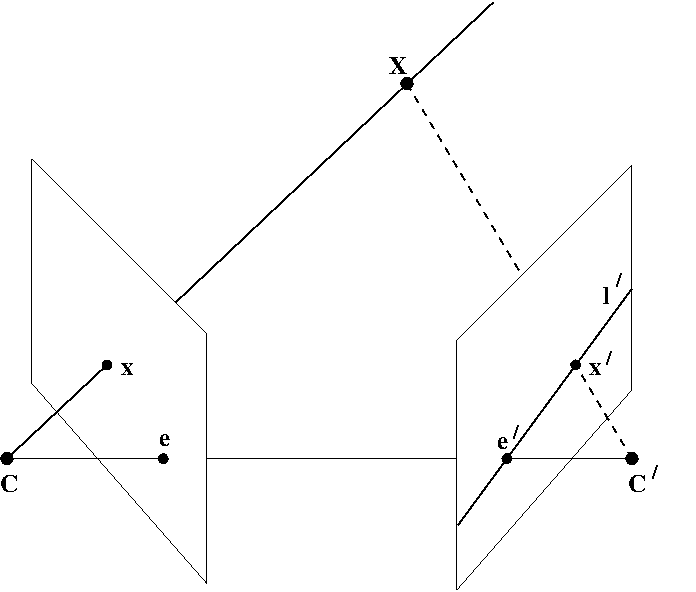
\includegraphics[scale=0.5]{pics/epipolar geometry.png}
		\caption{Эпиполярная геометрия} 
		\label{pic:epipol} % название для ссылок внутри кода
	\end{center}
\end{figure}

Таким образом, соблюдение указанных выше требований позволяет использовать следующий геометрический принцип. Пусть имеются две камеры, как изображено 
на рисунке \ref{pic:epipol}. $C$ — центр первой камеры, $C'$ — центр второй камеры. Точка пространства $X$  
проецируется в $x$ на плоскость изображения левой камеры и в $x'$ на плоскость изображения правой камеры. Прообразом точки $x$ на изображении левой 
камеры является луч $xX$. Этот луч проецируется на плоскость второй камеры в прямую $l'$, называемую эпиполярной линией. Образ точки $X$ на плоскости 
изображения второй камеры обязательно лежит на эпиполярной линии $l'$.
% TODO: таким образом повторяется -> ?
Таким образом, каждой точке $x$ на изображении левой камеры соответствует эпиполярная линия $l'$ на изображении правой камеры. При этом пара для $x$ на 
изображении правой камеры может лежать только на соответствующей эпиполярной линии. Аналогично, каждой точке $x'$ на правом изображении соответствует 
эпиполярная линия $l$ на левом.

Далее с помощью точек $x$ и $x'$ возможно посчитать смещения каждого пикселя одного изображения относительно другого, что даёт карту смещений (disparity map). 
Очевидно, что смещения будут подсчитаны только для точек, видимых обеими камерами. Карта смещений же приводится либо к облаку точек, либо к карте глубины. Пример
такой карты представлен на рисунке \ref{pic:depth} \cite{lipson2021raft}. 

%После нахождения карты смещения остаётся по известным внешним параметрам камер рассчитать глубину. Глубина каждой точки P, воспринимаемой двумя камерами 
%с оптическими центрами Ol и Or, определяется проекциями p, p' этой точки на каждый кадр. Тогда значение глубины по уравнению, указанному ниже []. 
%Z = f{T \over d},\eqno{\hbox{(2.1)}}
%где T - расстояние между Ol и Or;
%    d - смещение,  {d = x - x'};
%	f - фокусное расстояние камеры.

\begin{figure}[H]
	\begin{center}
		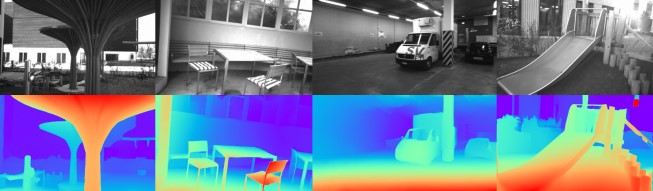
\includegraphics[scale=0.7]{pics/exmpl.jpg}
		\caption{Примеры результата работы} 
		\label{pic:depth} % название для ссылок внутри кода
	\end{center}
\end{figure}

На практике работу большинства алгоритмов можно разделить на 3 этапа: получение изображений, поиск соответствий и восстановление информации о глубине. Это позволяет
организовать классификацию алгоритмов на основе подходов к каждому из этих этапов. 
% получает два снимка с синхронизированных камер, решает проблему поиска соответствий для сопоставления пикселей на снимках, соответствующих 
%одной точке пространства и затем восстанавливает информацию о глубине. Результатом является карта глубины изображения или облако точек. 

\section{Восстановление}

Вообще восстановление из диспарити карты просто считается через фокус. Мб тут рассказать про методы повышения качества диспарити карт или борьбы с перекрытиями. Или про методы, не основанные на расхождениях. 
%% TODO: придумать, что писать, и написать это


\section{Поиск соответствий}

Как было ранее сказано, поиск соответствий можно выполнять широким набором методов. Цель каждого метода - постараться найти для каждого пикселя одной картинки 
соответствующий ему пиксель на второй. Достичь этого можно двумя подходами в зависимости от накладываемых ограничений на зону поиска соответствий.  При подсчёте 
расхождений лишь в небольшой окрестности или окне вокруг интересующего нас пикселя мы говорим о локальных методах, эти методы  используют небольшое количество 
информации и относительно быстродействены. Локальные методы в свою очередь делятся на три категории: block matching (сопоставление блоков?), градиентные методы и 
сопоставление особенностей (feature matching). 		//TODO: вставить правильный перевод

Глобальные методы же проводят поиск в целом ряде пикселей или во всём изображении. Они не так чувствительны к локальным дефектам, мешающим процессу поиска соответствий 
(например, заслонение), но при этом имеют куда большую вычислительную сложность. Одним из самых популярных подходов в этой группе методов является динамическое программирование, 
которое позволяет разбить вычислительно сложную задачу на множество простых подзадач \cite{dynamic_prog}.   	 

\subsection{Block matching}

BM - это локальный метод, который заключается в оценке расхождения в точке на одной картинке с помощью сравнения небольшой области вокруг этой точки с такими же областями 
на другой \cite{}. Благодаря выпрямлению (ректификации) поиск соответствующей области на другой картинке ограничивается одним измерением. По этому измерению (как правило, строке) 
считается одна из доступных метрик, и регион с наименьшим её значением считается искомым. Существует целый набор метрик, часто используемых в этом методе. 

Для отдельных пар пикселей можно рассчитывать абсолютную разность (AD) или квадратичную разность (SD), выраженную через их интенсивности:
\begin{equation}
	AD(x, y, d) = |I_l(x,y) - I_r(x+d, y)|,			
	\label{eq:AD}
\end{equation}
где $(x, y)$ - координаты первого пикселя; $d$ - сдвиг по оси x между двумя пикселями или диспаритет; $I$ - интенсивность данного пикселя. Обычно $I_l$ обозначают опорное изображение, а $I_r$ - 
целевое. Абсолютная разность - простейшая метрика, за счёт чего до сих пор используется в многих алгоритмах, от которых требуется производительность в реальном времени []. 

Для квадратичной разности 
\begin{equation}
	SD(x, y, d) = |I_l(x,y) - I_r(x+d, y)|^2.		
	\label{eq:SD}
\end{equation}

На основании этих метрик были выведены более точные и сложные, такие как сумма квадратичных разностей (SSD) и сумма абсолютных разностей (SAD). Они применяют описанный выше принцип для целого 
окна пикселей вокруг исследуемого.  Благодаря всё ещё достаточно высокой скорости работы эти метрики позволяют повышать качество итоговой карты смещений за счёт варьирования размера окна и 
дополнительных проходов по изображениям \cite{twosizewindow} 

Также применяется нормированная кросс-корреляция (NCC) - стандартный статистический метод для поиска соответствий с шаблоном, который записывается для случая поиска соответствий пикселей 
согласно уравнению \ref{equ:NCC}.

\begin{equation}
	NCC(x, y) = \frac{ \sum_{x, y}^{} (I_l(x, y) - \overline{I_l} )^2 * ( I_r(x + d, y) - \overline{I_r} )^2   }{ \sqrt{ \sum_{x, y}^{} (I_l(x, y) - \overline{I_l} )^2 * ( I_r(x + d, y) - \overline{I_r} )^2 }  }, 
	\label{equ:NCC}
\end{equation}

где $\overline{I_l}$ и $\overline{I_r}$ - средние интенсивности соответствующих изображений. Эта метрика устойчива к перепадам яркости и контрастности изображения благодаря нормализации \cite{ncceval}, 
но требует выполнения значительно большего числа арифметических операций. 

\subsection{Feature matching}

Довольно распространёнными являются методы, основанные на использовании характерных точек - методы SIFT \cite{}, SURF \cite{} 
и методы, основанные на детекторах Харриса и других. Различным способам поиска этих характерных точек посвящено немало статей. 

Суть методов, относящихся к этой группе, заключается в выделении на снимках характерных точек: углов и точек смены контраста. Далее 
для найденных точек считается дискриптор - вектор, являющийся численной характеристикой окрестности характерной точки. Таким образом,
установление соответствий сводится к сравнению численных величин этих векторов. 

Новые работы в этой области продолжают публиковаться. Так был предложен метод на основе SIFT, использующий самоорганизующиеся карт для 	% TODO: почитпть про эти карты
достижения более высокой производительности \cite{modsift}. Работа Liu и других \cite{ekstrand2015high} же опирается на использование комбинации из сегментации 
изображения и обнаружения границ в качестве метрики поиска совпадений. Такая реализация работает быстро, но точность результатов по=прежнему остаётся
невысокой, особенно в областях прерывистости. % discontinuity

Метод менее чувствителен к перекрытиям и слаботекстурированным областям, 
но, к сожалению, плотность точек, для которых возможно подсчитать глубину, получается относительно низкой, что привело к снижению интереса 
к этой группе методов.

\subsection{Градиенты }

% ГЛОБАЛЬНЫЕ
\subsection{Методы динамического программирования}

\subsection{Graph cut}



\section{Получение изображений}

\subsection{Стерео одной камерой }

\subsection{Fisheye-stereo}


\section{Выводы}


\newpage
\bibliographystyle{plain}
\bibliography{refs}

\end{document}
